In figure \ref{img:analysis} is described the first phase of a project,
regarding requirements analysis, as seen form AllSpark inside perspective.
Figures \ref{img:allocate} and \ref{img:gathering} explain in details the 
subprocesses called from the main process.
These, respectively, describe the procedure followed for allocate
a project and the relation between AllSpark and the consumer while collecting 
the requirements for the project.
\paragraph{}
Figure \ref{img:deploy} illustrates the business process which covers the last
phase of a project development: the effective deployment of the product.


\begin{figure}
\centering
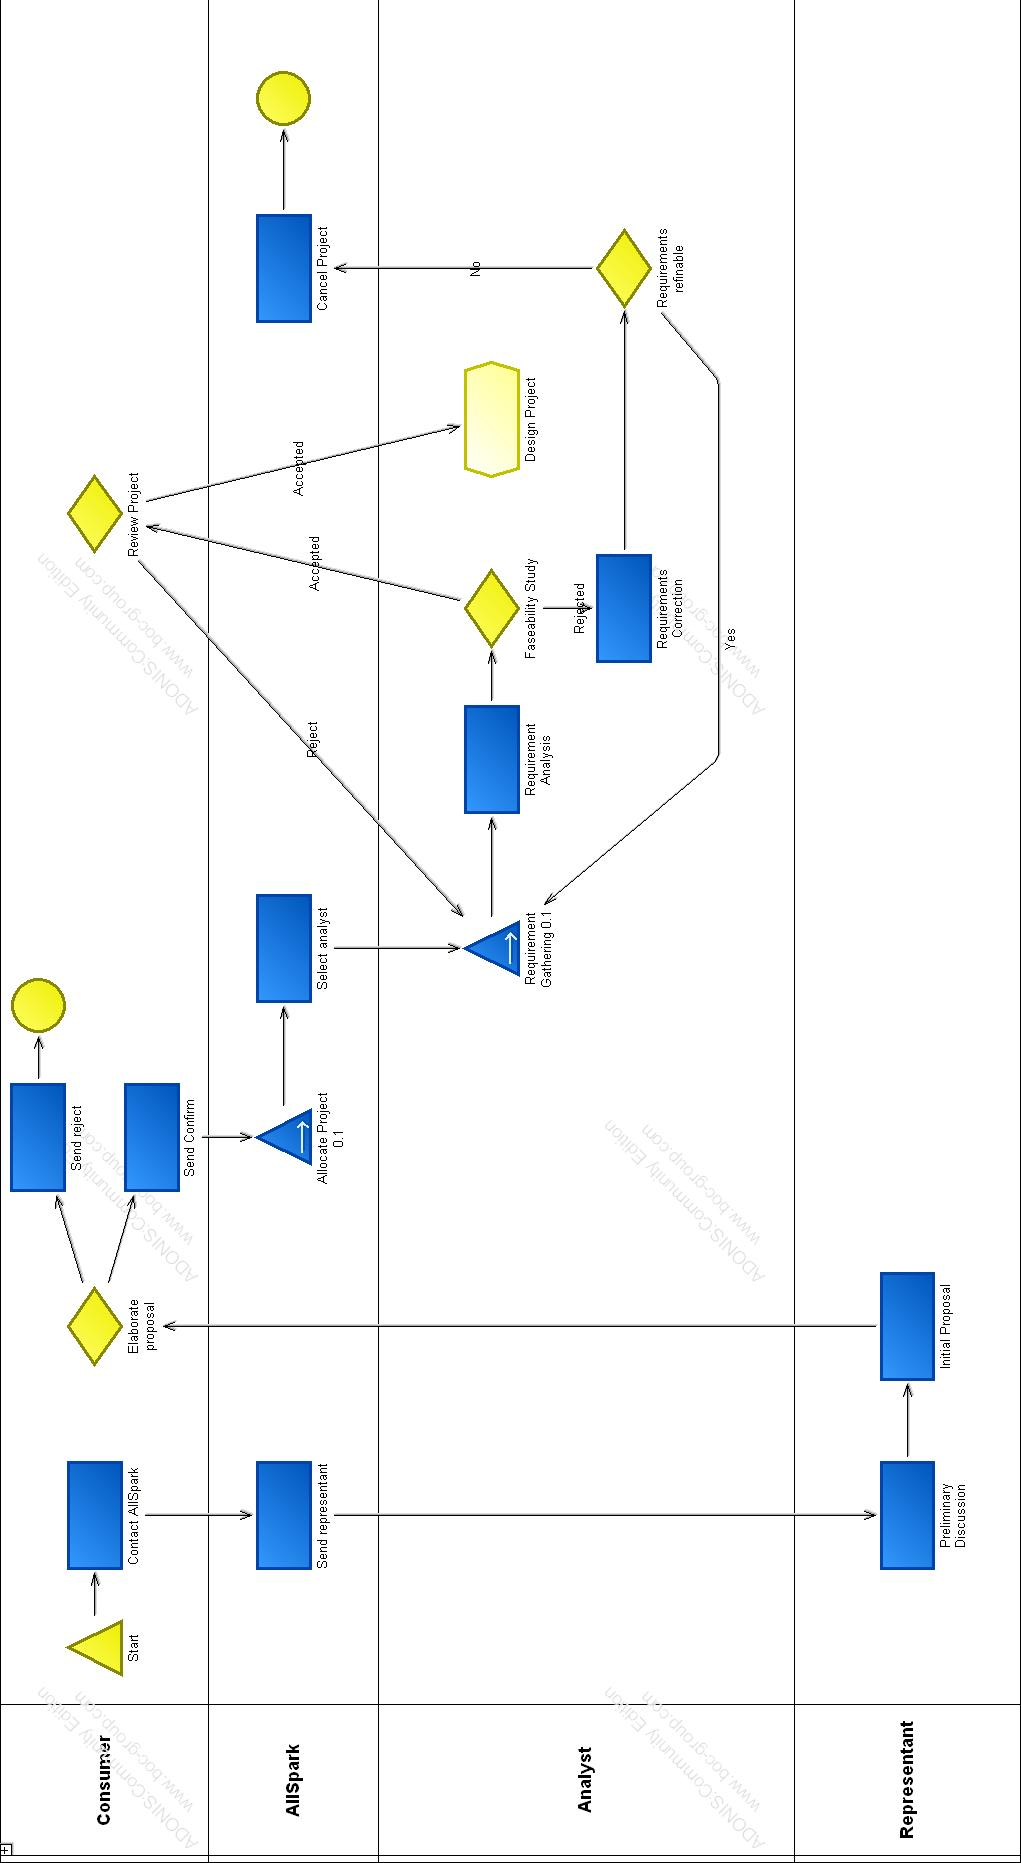
\includegraphics[scale=0.30]{adonis_diagrams/analysis}
\caption{Business process describing the first phase of a project development}
\label{img:analysis}
\end{figure}

\begin{figure}
\centering
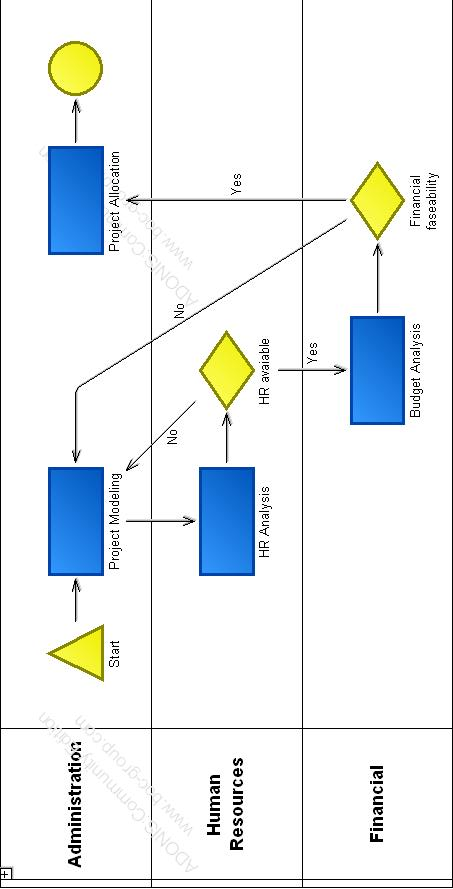
\includegraphics[scale=0.50]{adonis_diagrams/allocate}
\caption{AllSpark procedure for project allocation}
\label{img:allocate}
\end{figure}

\begin{figure}
\centering
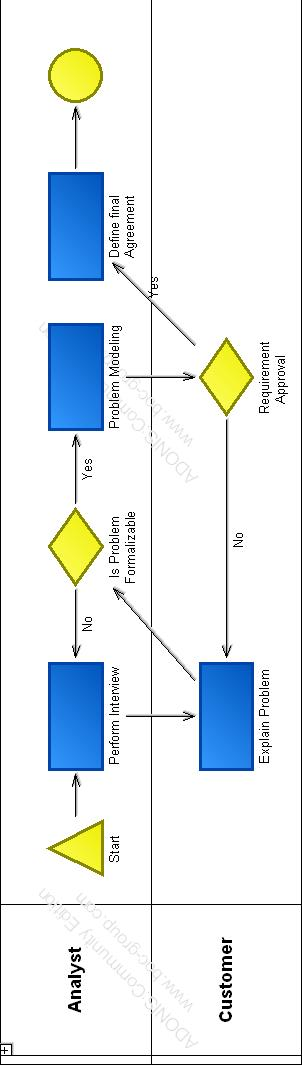
\includegraphics[scale=0.50]{adonis_diagrams/gather}
\caption{AllSpark procedure for requirements gathering}
\label{img:gathering}
\end{figure}

\begin{figure}
\centering
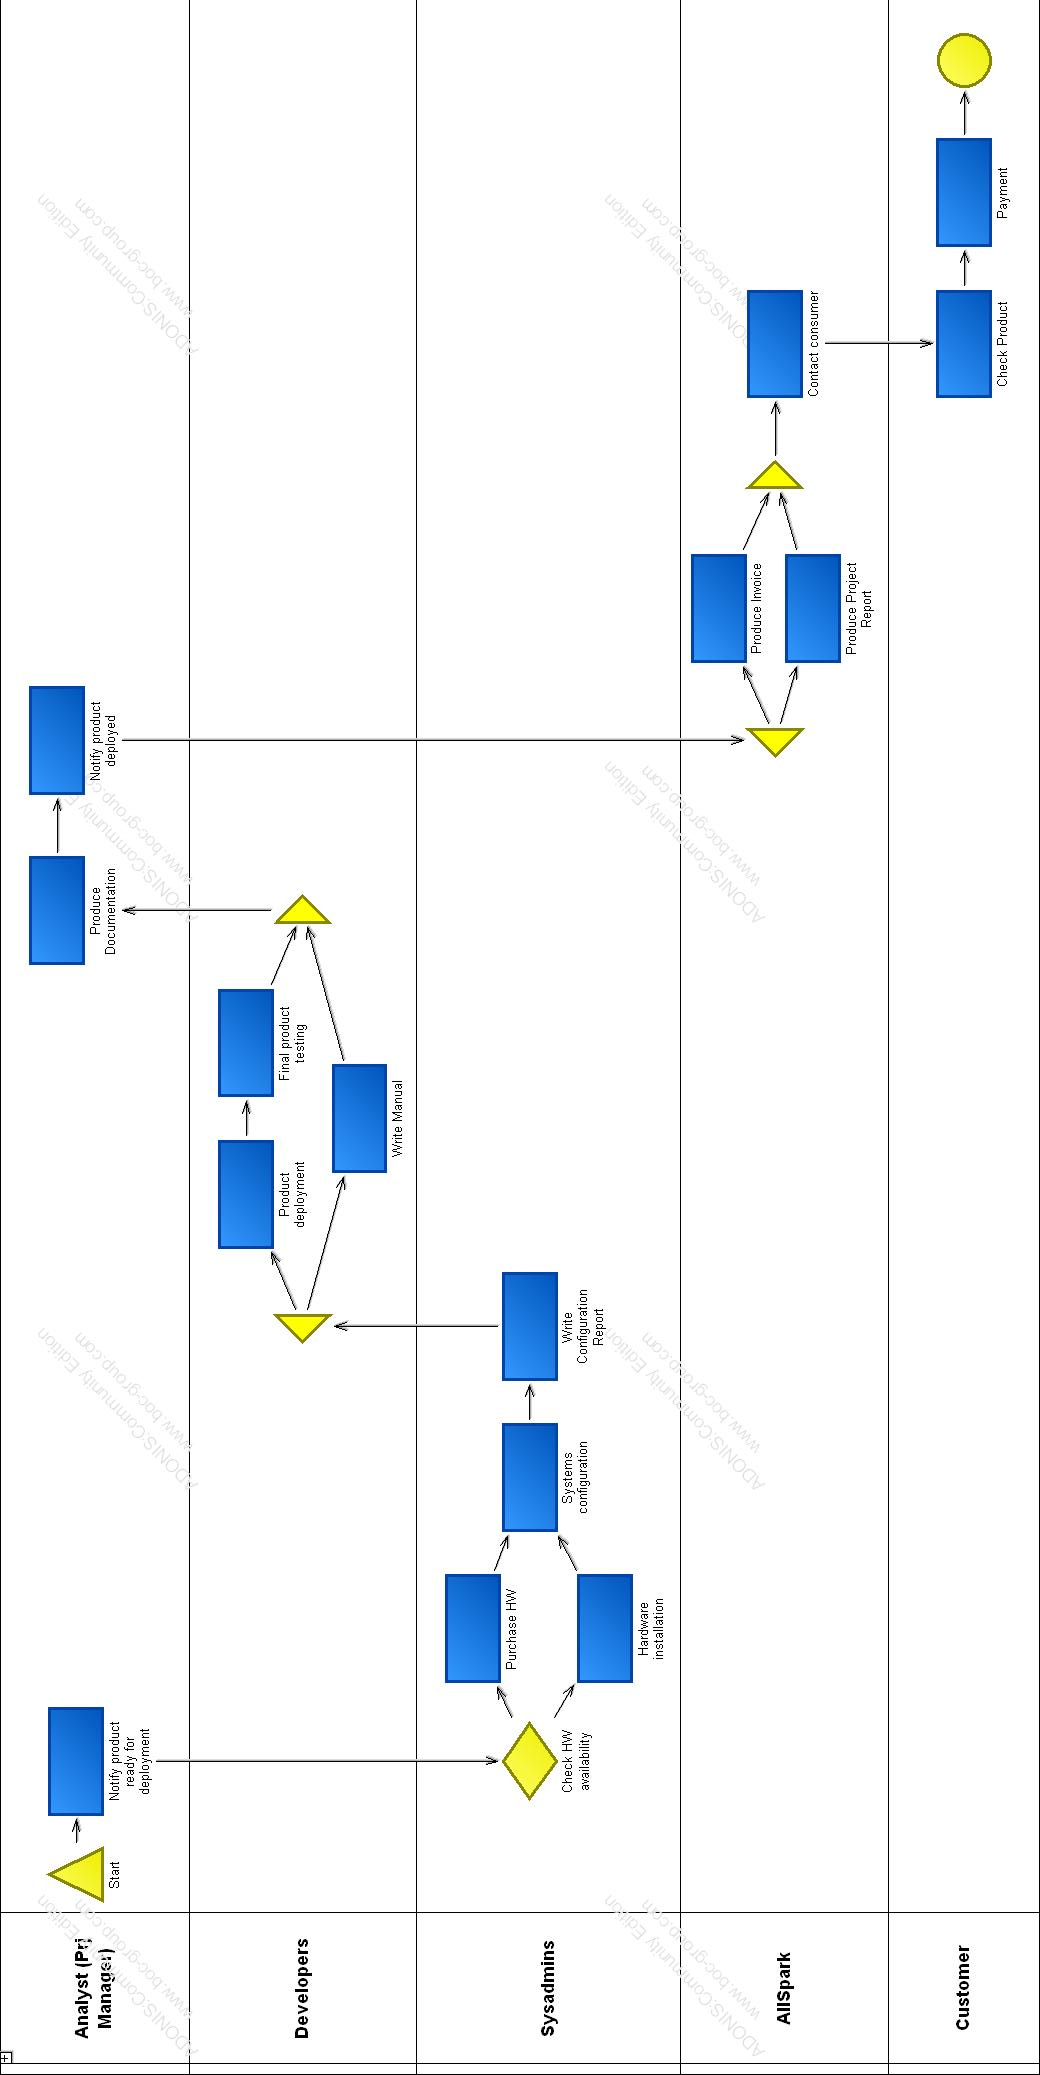
\includegraphics[scale=0.27]{adonis_diagrams/deploy}
\caption{Deploying of a project}
\label{img:deploy}
\end{figure}
